% LDV Vorlage zuerst installieren
% Zip verfügbar unter: https://www.ldv.ei.tum.de/studentische-arbeiten/
%
% Alternative Typen von Abschlussarbeiten
%   doctype=Studienarbeit
%   doctype=Bachelorthesis
%   doctype=Diplomarbeit
%   doctype=Mastersthesis
%
% Sprachen
%   ohne lang-Attribut:  Englisch
%   lang=ngerman:        Neue deutsche Rechtschreibung
\documentclass[doctype=Studienarbeit,oneside]{ldvbook}

% !TeX spellcheck = en_US

\usepackage{float}
\usepackage[justification=centering]{caption}

\begin{document}

\subject{Advanced Seminar}
\title{uFixit - Augmented Reality Manuals}
\subtitle{An AR Product Concept}
\author{Manuel Kimmel, Stefan Urban, Firas Zoghlami}
\license{CC-BY}
\supervisor{Dr. Hao Shen}
\date{July 13, 2016}

\maketitle


\chapter*{Abstract}

Eine Zusammenfassung der Problemstellung und der wichtigsten
Ergebnisse auf maximal einer Seite.


\tableofcontents


% !TeX spellcheck = en_US

\chapter{Introduction}
	
	problem: "things" get more complicated each day. additionally, these last years, repairing stuff has become nearly impossible.
	
	\begin{itemize}
		\itemsep0em
		\item mobile phones get less and less parts > even batteries are not replaceable anymore
		\item cars include expensive electronics in every single part
		\item solely from mechanical party consisting products are most likely made out of cheap irreplaceable plastic parts
	\end{itemize}
	
	solution:
	\begin{itemize}
		\itemsep0em
		\item find a professional (expensive)
		\item repair the thing yourself \begin{itemize}
			\itemsep0em
			\item with the help of the manufacture \begin{itemize}
				\item not really wanted > a repaired product last longer and shrinks profits from selling new product
				\item nowadays only for professional equipment (business laptops, ...)
					\begin{figure}[H]
						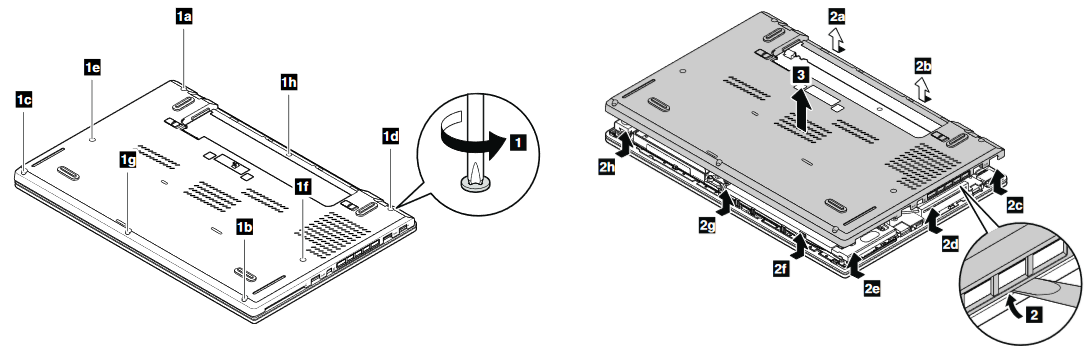
\includegraphics[width=\textwidth]{../images/common-manual.png}
						\centering
						\caption[adsf]{Typical step-by-step manual for business laptop hardware, taken from Hardware Maintainance Manual by Lenovo Thinkpad\footnotemark}
					\end{figure}
					\footnotetext{\url{https://download.lenovo.com/ibmdl/pub/pc/pccbbs/mobiles_pdf/t440s_hmm_en_sp40a25360_04.pdf}}
			\end{itemize}
			\item without the help of the manufacture \begin{itemize}
				\itemsep0em
				\item with technical skills > requirements increase drastically
				\item with no technical skills > manuals by other users (youtube videos, ...)
			\end{itemize}
		\end{itemize}
	\end{itemize}
	
	OUR solution:
	\begin{itemize}
		\itemsep0em
		\item \textbf{help user with repairing things by their own}
		\item new approach: use AR
		\item AR will come into the houses over the next years > device available
		\item AR devices are designed to show/add information to your environment and at the same time keep your hands free (alternation and interaction possible!) (not for tablets, ...) ...
	\end{itemize}
	
	
	section 2 will deal with the general product idea.
	
	section 3 takes a look at the specific problems that have to be faced because we use augmented reality
	
	section 4 checks possible business opportunities
	
% !TeX spellcheck = en_US

\chapter{Concept Description}

	uFixit is a platform on which users can get repair manuals. It does not matter from which manufacturer it comes, it works with all products of any brand. There is only one minor constraint: The part has to be fixable.
	
	\begin{figure}[H]
		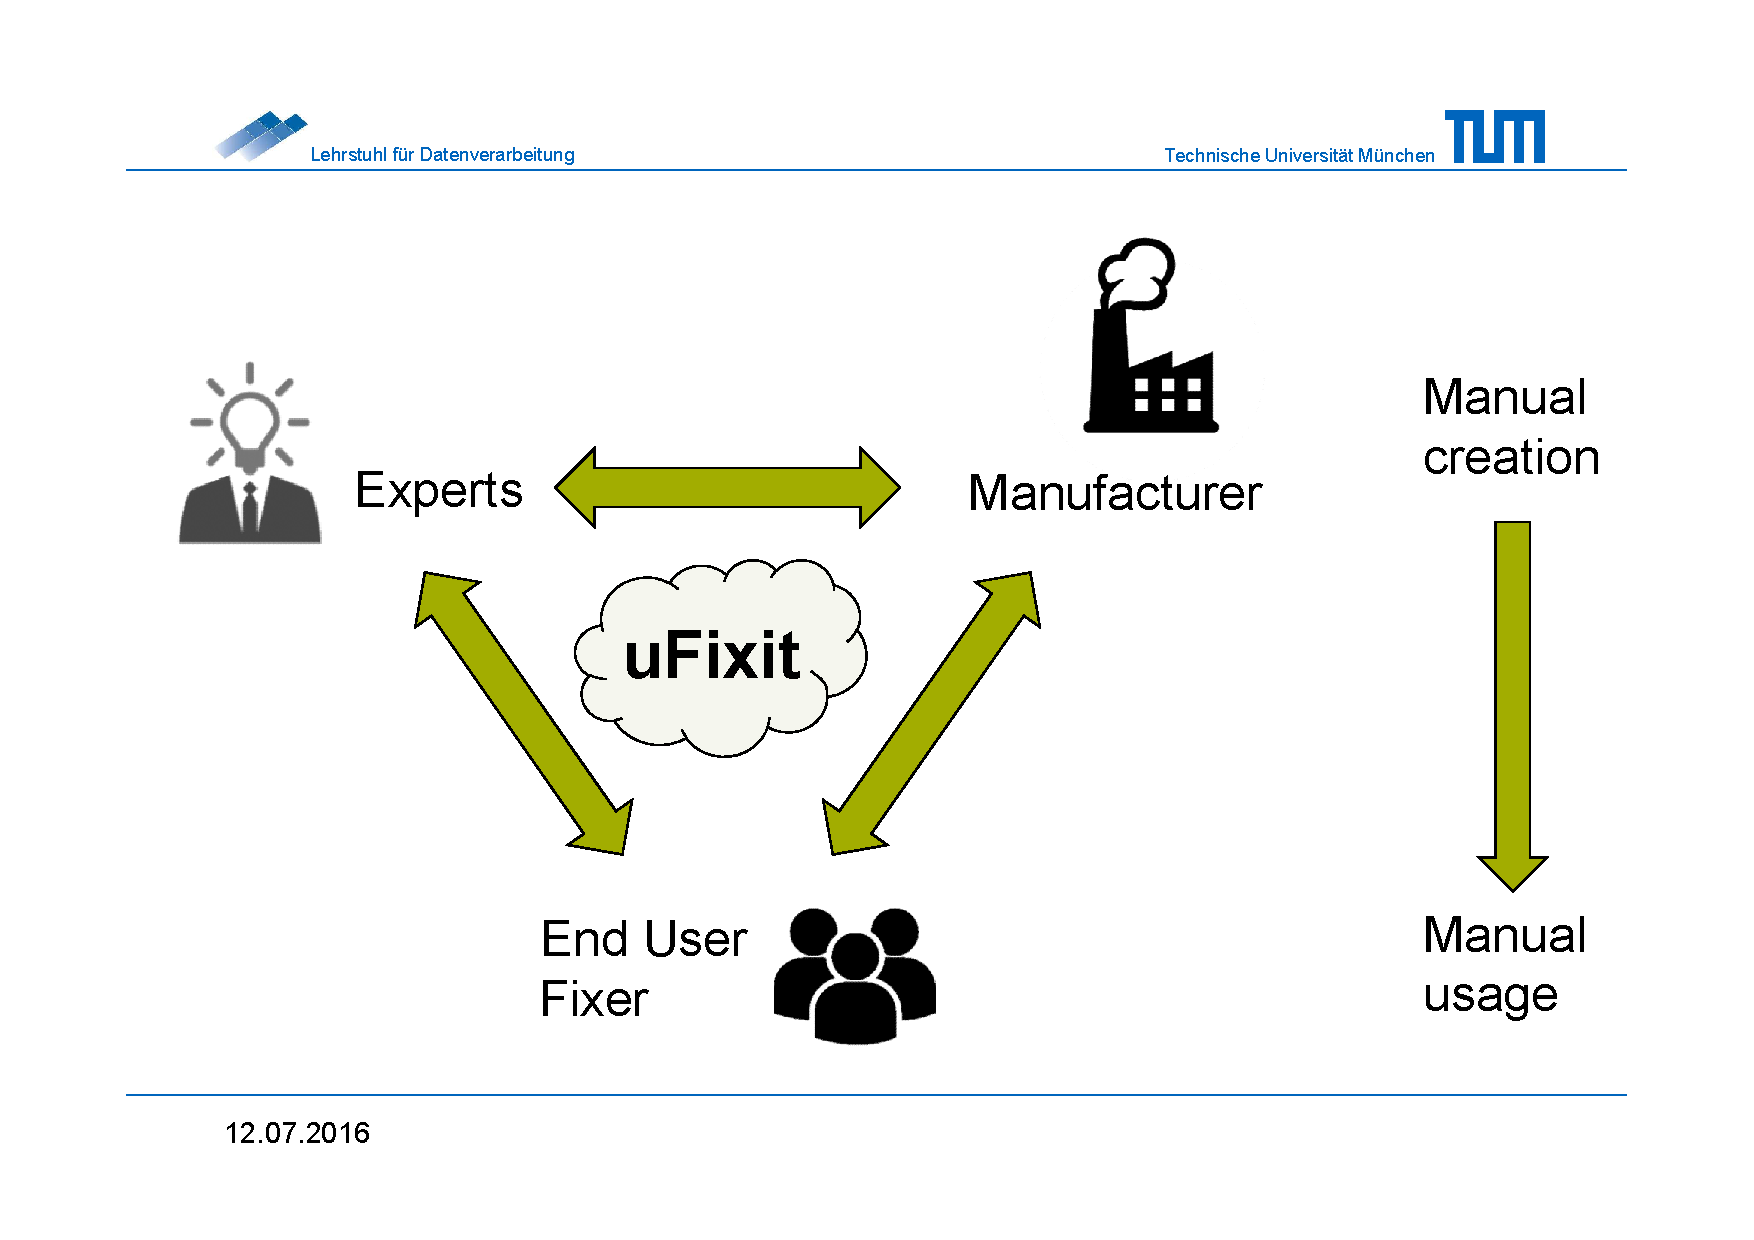
\includegraphics[width=\textwidth, trim=0cm 3cm 0cm 4cm, clip]{../images/involved-parties.pdf}
		\centering
		\caption{Parties involved in the uFixit environment}
		\label{fig:involved-parties}
	\end{figure}

	As one can see in \autoref{fig:involved-parties}, \textbf{Experts} and \textbf{Manufacturers} create the manuals, whereas \textbf{Fixers} use them to repair items. An Expert is a person that has the same equipment as an end user, but uses it to create manuals. He will not have special training or software to do so. Manufacturers on the other side have detailed information and models of their products and therefore can develop high quality instruction steps with animations and extensive highlighting.
	
	After describing how the instructions inside a manual looks like, we discuss how uFixit helps experts as well as manufacturers in creating the best possible manuals for the end user. For the conclusion of this chapter we have a look at how the experts are motivated to create content for our platform.


	\section{Instructions format}
	\label{sec:instr-format}
	
		Every manual is separated into several individual steps. The first step is always the diagnosis because to do the repair itself, we do need to know what is broken. While holding the defective part into the FOV of the camera, uFixit will try to match it to an internal database. If this succeeds, the next step is to get the right manual and suitable tools.
		
		
		After the preparation phase, the actual repair process begins. In each step, the user will be asked to perform a specific task. Subsequently the manual moves to the next step. This is executed in the following ways:
		
		\begin{itemize}
			\itemsep0em
			\item The AR device constantly watches the fixer while performing the task. With the help pf tracking algorithms, the application can detect when a step is finished and will automatically jump to the next one.
			\item Ideally the used device has a microphone built in. With that, the fixer simply can issue a voice command.
			\item Although it is more of a feature to jump to a specific step in the tutorial, forward and backward buttons are provided on screen for easy access.
		\end{itemize}
		
		\begin{figure}[H]
			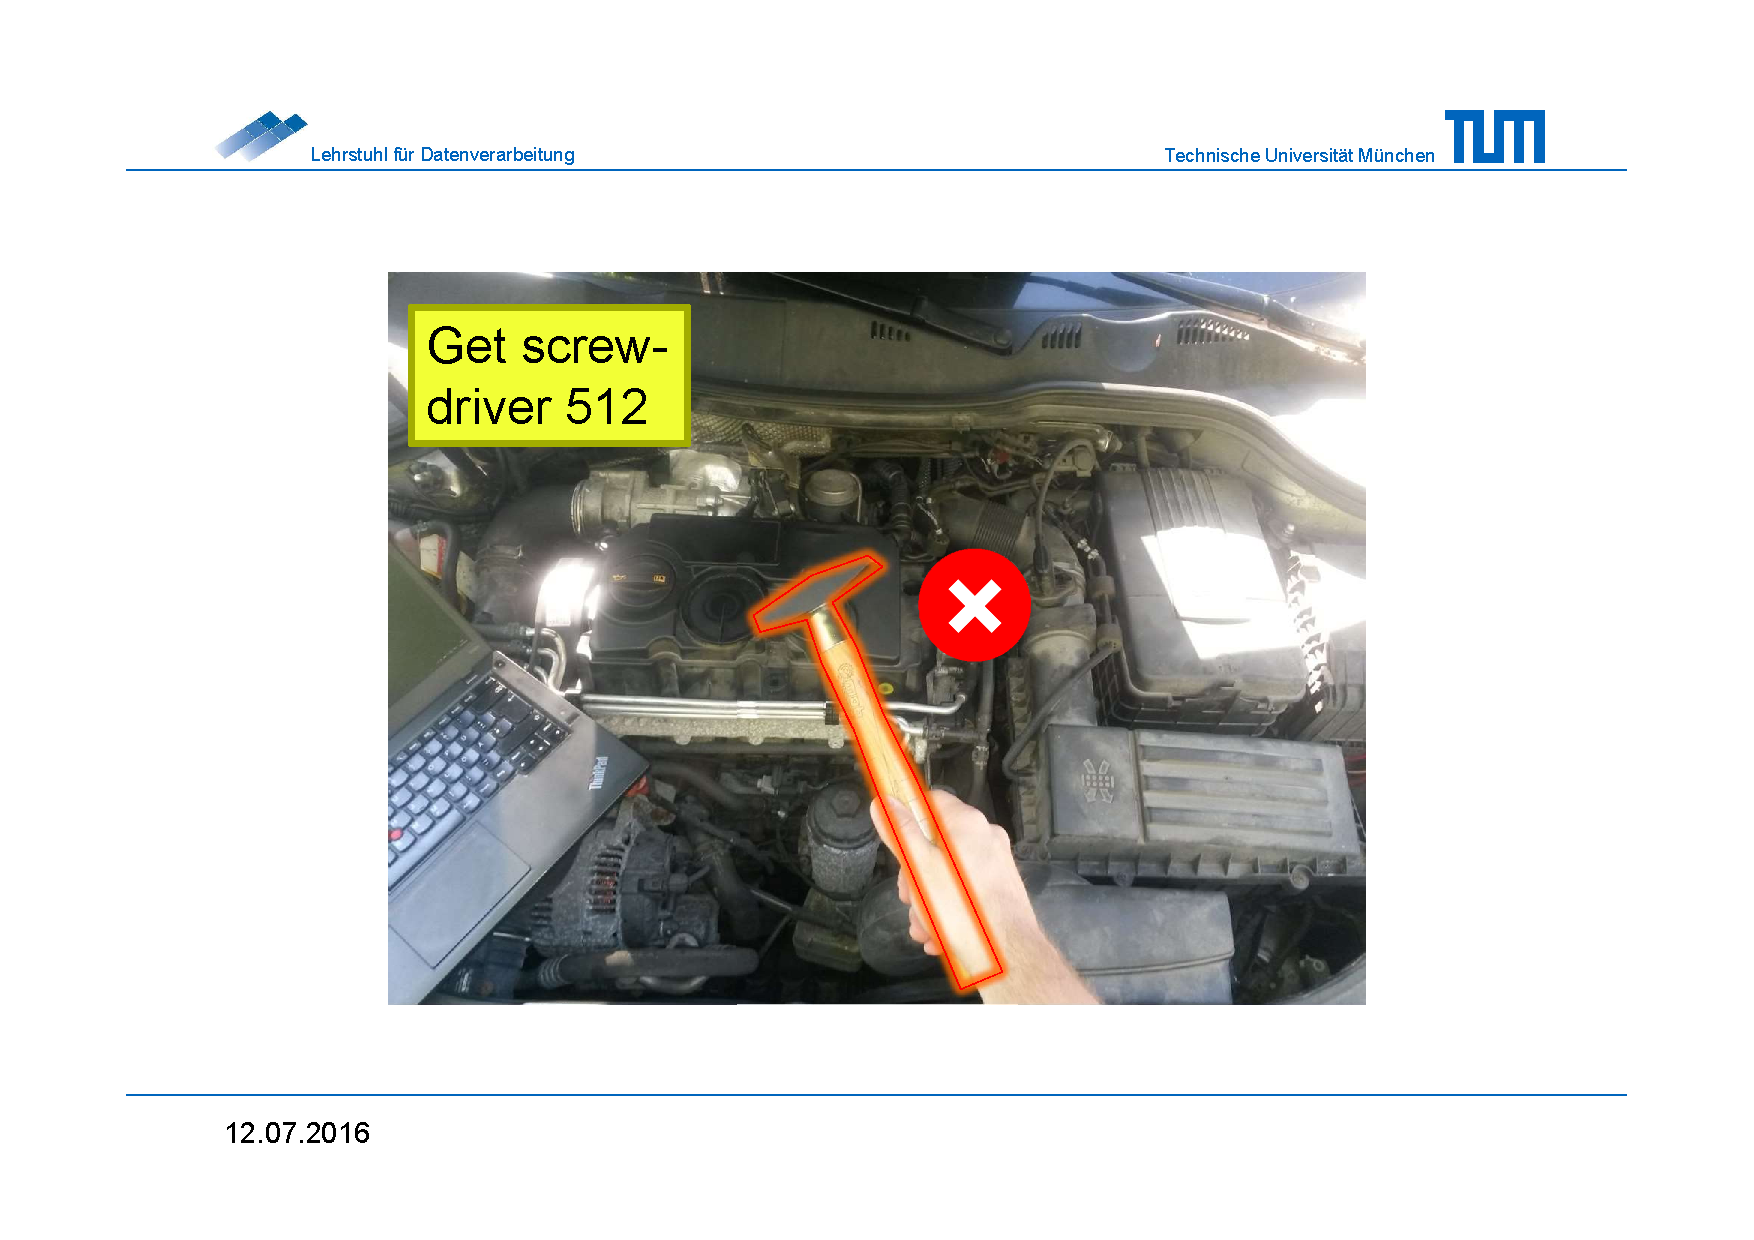
\includegraphics[width=\textwidth, trim=4cm 3cm 4cm 4cm, clip]{../images/instr-hammer.pdf}
			\centering
			\caption{Application is highlighting the wrong tool with a flashing read shadow}
			\label{fig:instr-hammer}
		\end{figure}
		
		\begin{figure}[H]
			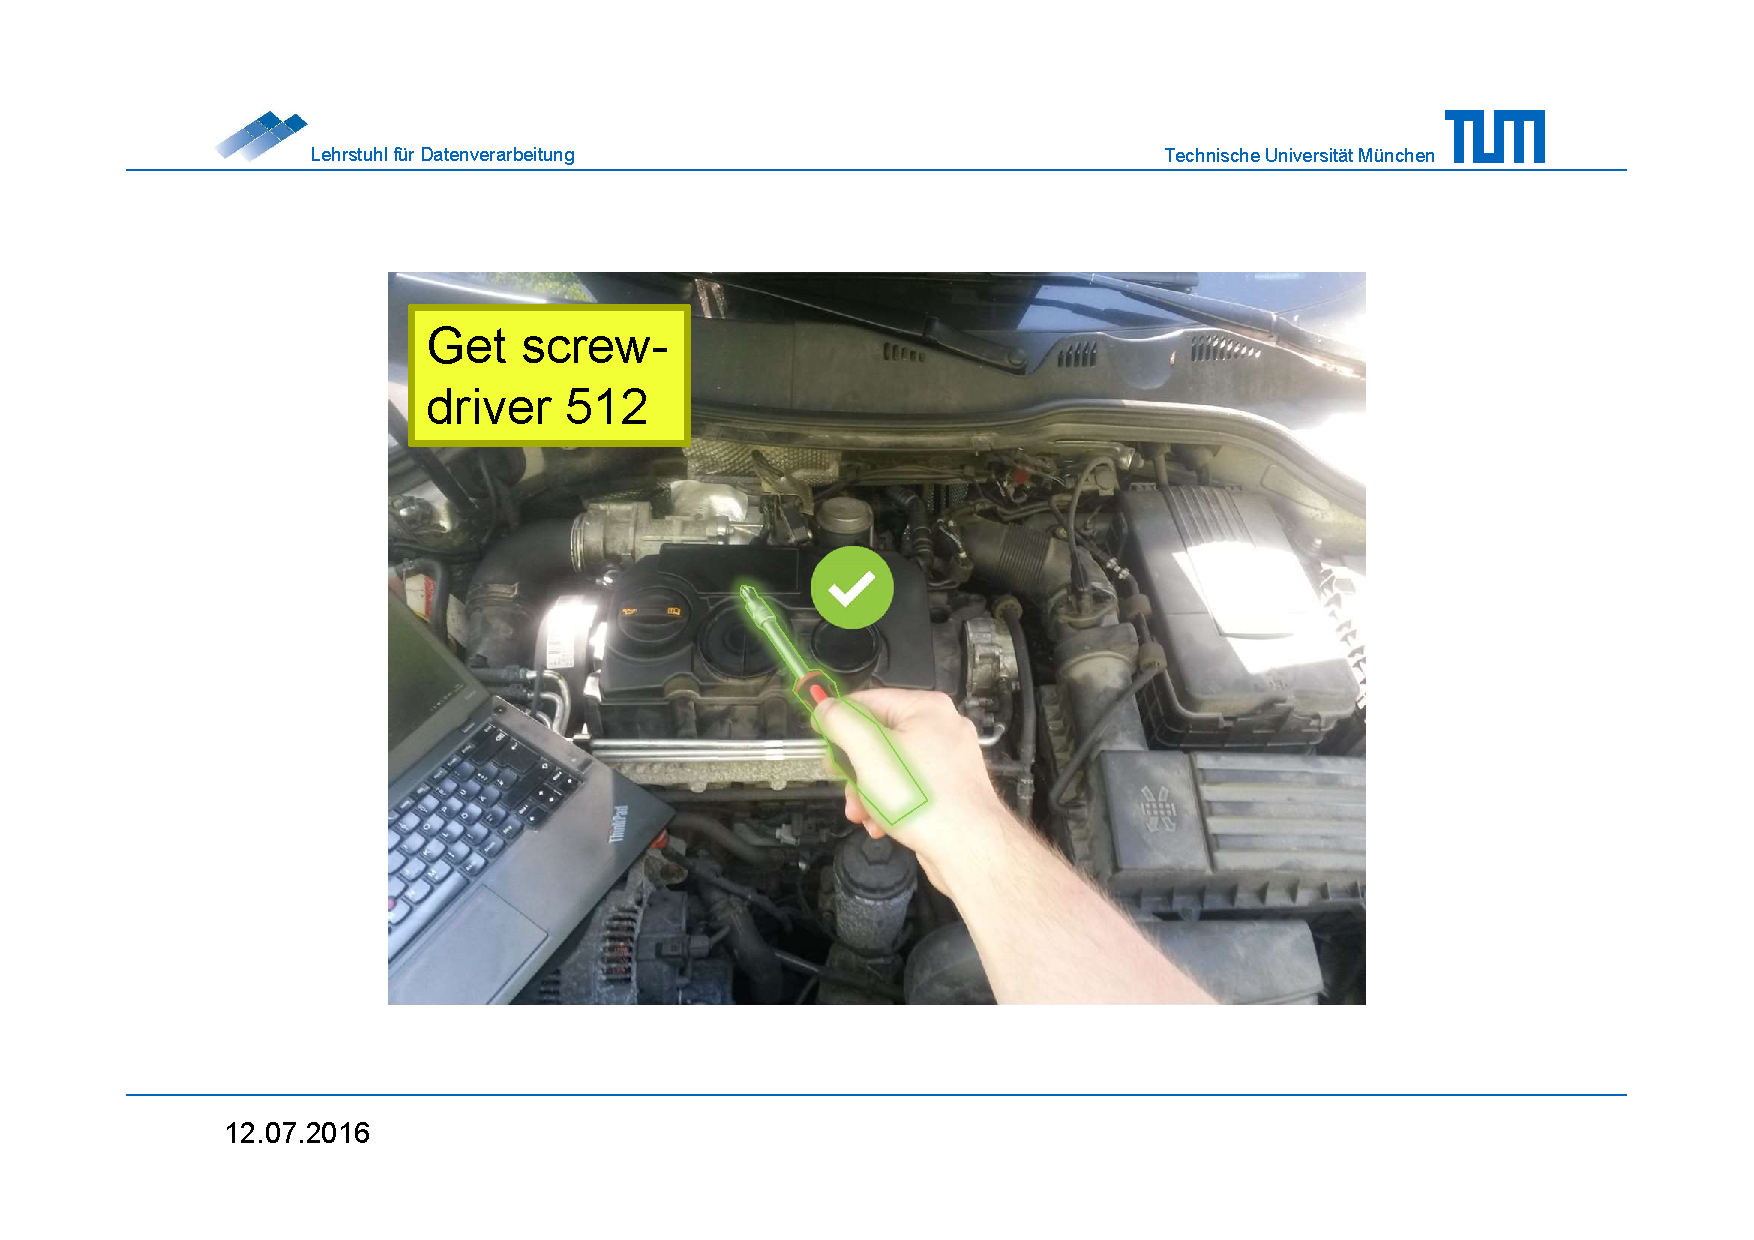
\includegraphics[width=\textwidth, trim=4cm 3cm 4cm 4cm, clip]{../images/instr-screwdriver.pdf}
			\centering
			\caption{When the Fixer picks up the right tool, the application will highlight it with a green shadow and after a short time transition to the next step}
			\label{fig:instr-screwdriver}
		\end{figure}
		
		\autoref{fig:instr-hammer} and \autoref{fig:instr-screwdriver} show how one instruction step looks like. The current task is shown in the top left - here: "Get screwdriver 512". When the user holds up a hammer, the AR device will register that and tell him that he is holding the wrong tool. After getting up the right tool, the manual will continue to the next step automatically.
		
	
	\section{Using existing AR Hardware devices}
	
		One of the clous abouts uFixit is that the fixer can use almost every AR device on the market. It only has to fulfill a certain list of requirement that are described in chapter 3. Although users will get the most excellent experience with AR head mounted devices like the Microsoft HoloLens or the Meta 2 (\autoref{fig:meta2}), other devices like smartphones are also supported.
		
		\begin{figure}[H]
			\centering
			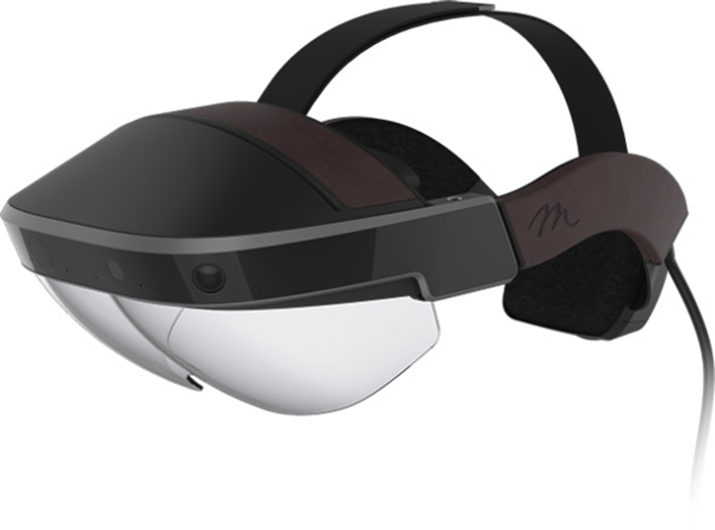
\includegraphics[width=0.5\linewidth]{../images/meta2.png}
			\caption{Meta 2 - Only one of the several devices uFixit will support}
			\label{fig:meta2}
		\end{figure}
		
		One outstanding example of this kind, which will receive special support, is Google's Project Tango. This is basically an augmented reality platform definition for Android based phones and tables.
		
		\begin{figure}[H]
			\centering
			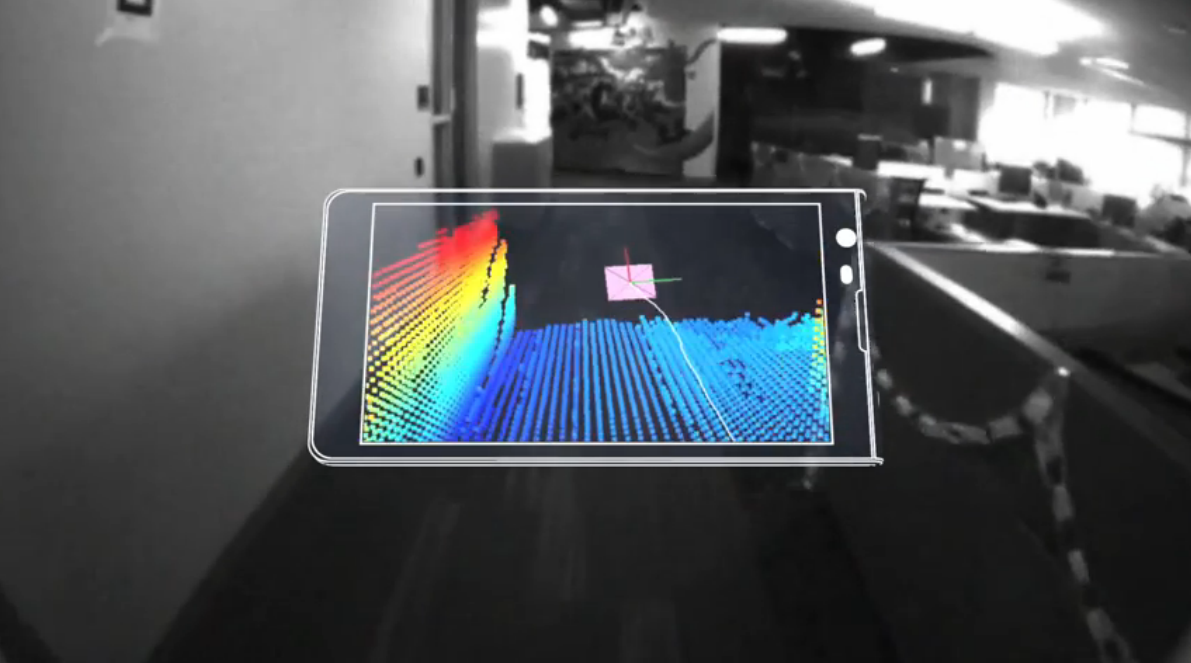
\includegraphics[width=0.7\linewidth]{../images/project-tango}
			\caption{Registration visualized using Project Tango by Google}
			\label{fig:project-tango}
		\end{figure}
		
		Of course if one does not have a suitable device, the manuals always can be watched using a webbrowser on a web portal as simple classical pages.
		
	
	\section{Software}
		
		Besides the application targeted for the end user, the Fixer app, there are two additional ones that provide content for the first one. They can be seen in \autoref{fig:software-overview}.
		
		\begin{figure}[H]
			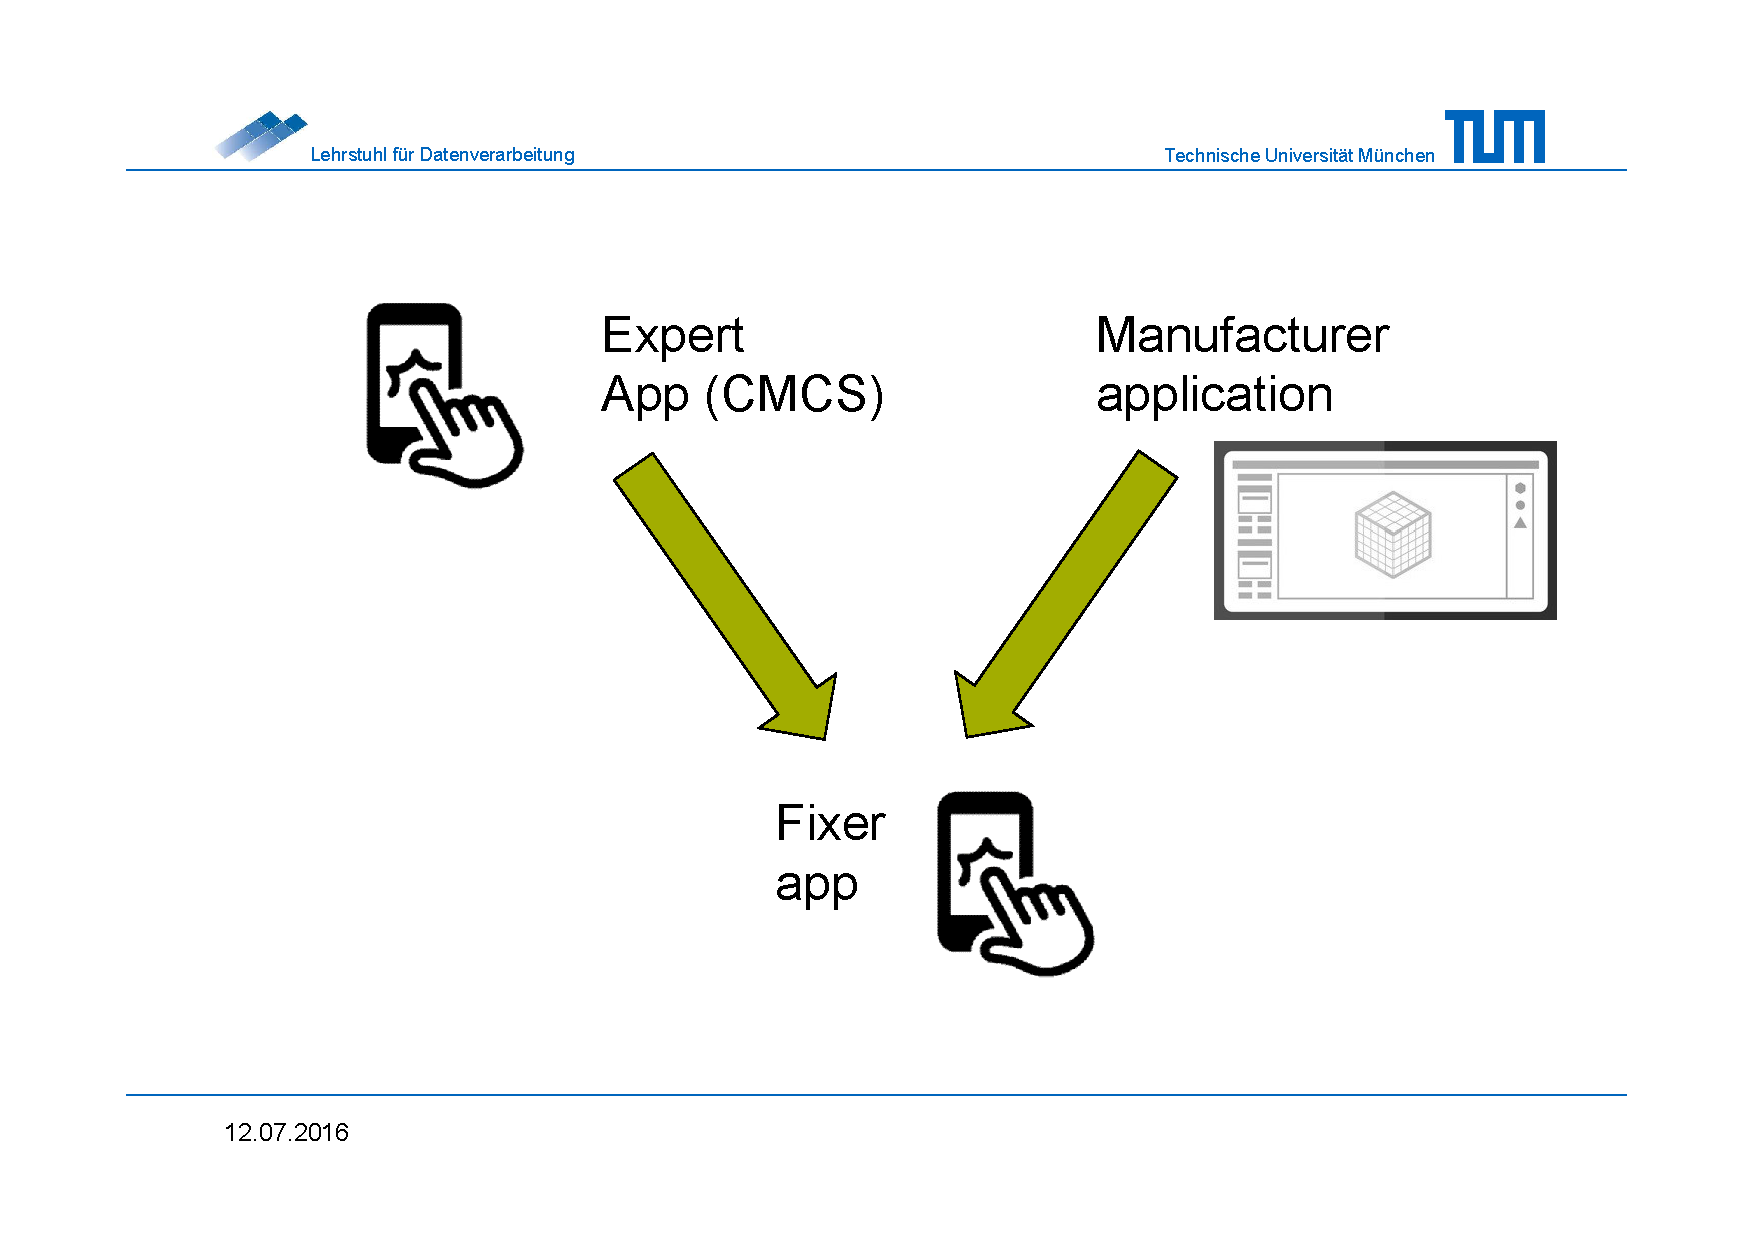
\includegraphics[width=\textwidth, trim=4cm 3cm 3cm 4cm, clip]{../images/software-overview.pdf}
			\centering
			\caption{uFixit applications Eco-system}
			\label{fig:software-overview}
		\end{figure}
		
		The Experts are creating their manuals with a simple, intuitive and fool proof app on the same AR devices the Fixer uses. It is called \textbf{Community Manual Creation Software} (CMCS). The main goal is to make creating manuals available for everybody. One can only use the application itself or - as described in (3.2.3) - use print-out markers to support correct annotation and arrow placement.
		
		Manufacturers will receive plugins for the various 3D CAD programs to seamlessly integrate with their already existing environment. Naturally the exported steps can be as complex as the manual engineer likes. Especially the things that can not be done with the Community Manual Creation Software are the most interesting:
		
		\begin{itemize}
			\itemsep0em
			\item animations
			\item see through content
			\item user defined masking of obscuring parts
		\end{itemize}
		
		Since every single AR device is unique in its own way, the \textbf{Fixer app} will provided a intuitive workflow specific to the device it runs on. It will still follow these three steps:
		
		\begin{enumerate}
			\itemsep0em
			\item Diagnosis: Find out what product the user wants to repair and how it is broken.
			\item Preparation: Obtain tools and manuals for next step
			\item Actual repair as described in \eqref{sec:instr-format}
		\end{enumerate}
		
		
	\section{Experts Reward Program}
	
		uFixit relies heavily on the Fixers to get involved in the community and to start creating own manuals. This can solely be based on idealism. Believing this would work on the other hand is pretty naive. Our solution: Money!
		
		Many big software companies nowadays have something called bug bounty program. This means if a person finds a bug of a certain severity in the manufacturer’s product, he will get rewarded when reporting it. This is very convenient for the company considering they do not have to pay everyone that is searching for these flaws in the software.
		
		We want the same principle integrated into uFixit. Experts should be lured into a \textbf{manual bounty program} that will reward them every time a Fixer solves a problem using his tutorial. The money will come from the manufacturer who will benefit from only paying a small amount for high quality content rather to spend more for trained personal..
	
	\section{Feedback}
	
		To provide the user with highest quality manuals, there will be an opportunity to rate them within a review system. Online shopping nowadays would be unimaginable without reviews just because no one likes to buy untested stuff. Especially when the end user needs quick and good help, he might invest in a manual that has a 100\% rating instead first trying the free one, with 75\% rating.

		\begin{figure}[H]
			\centering
			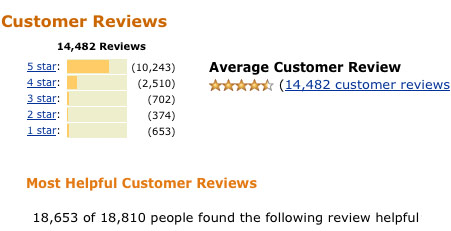
\includegraphics[width=0.7\linewidth]{../images/how-to-get-amazon-reviews-kindle.jpg}
			\caption{Example of product reviews on \url{amazon.com} with a overwhelming good average rating}
			\label{fig:amazon-reviews}
		\end{figure}
		
		\autoref{fig:amazon-reviews} is a screenshot from the \url{amazon.com} website. It shows a product review page with an overwhelming good average rating. Most of the users would now be convinced this is a great product and buy it without further research or thinking. the uFixit review system will be quite similar to this one because it will increase community involvement and building.

% !TeX spellcheck = en_US

\chapter{AR specific problems regarding realization}

\section{Hardware}
\label{sec:hardware}
As uFixit only provides the software solution for interactive manuals, the user is free to choose, which kind of AR hardware he would like to use for the application. To make the selection process easier, we first specify the requirements that the hardware has to fulfill and then propose two possible hardware solutions that are compatible with uFixit.

\subsection{Requirements}
Although there is no specific augmented reality hardware that is required to run uFixit manuals, a few requirements have to be fulfilled.

Firstly, the hardware has to be \textbf{mobile}, so that the user can take the instructions to the item he wants to repair. This is especially important if the item in question is too heavy to be moved, or is firmly mounted to its location. Therefore, the uFixit hardware has to be small and light enough to be carried around and also has to assemble and disassemble quickly.

This also rules out head tracking systems for the augmented experience, which require the installation of tracking cameras around the user to follow his head movements. Instead, a high resolution \textbf{RGB camera} is used for the object detection and an optional \textbf{depth camera} provides the exact distance between the observed object and the uFixit hardware.

Another important factor is, that many repairing tasks, require both hands to be executed. Therefore, the augmented reality device has to be \textbf{worn on the head}, so that the user can see the instruction manual all the time, without holding the device in one hand. This also requires a \textbf{lightweight} hardware solution, as the whole weight is carried only by the head.

If the current step of the manual is completed by the user, the next step is selected by speech commands. Speech control is the only suitable way for navigating through an uFixit manual, because it requires no hand interaction and therefore lets the user concentrate on the task. This means, that the hardware also has to supply a \textbf{microphone} to pick up the user commands.

The last requirement regarding the \textbf{computational power} of the device, is a not very restrictive. As uFixit essentially replays previously defined sequences of markers and overlays, the main computational effort lies in the real time object detection and to match those augmentations with the real world. This task is already executed by the hardware used in today’s mobile phones and therefore is not a limitation for the hardware selection process.

\subsection{Hardware Proposals}
Now we propose two already existing hardware solutions, which are guaranteed to be compatible with the uFixit application. 

The first one is the "Meta 2", a lightweight optical see through glass with an integraded 720p camera and a 3D depth sensor. It also has additional sensors for head movement tracking, which support the optical camera tracking via sensor fusion. The downside is, that the "Meta 2" has no integrated processor and has to be connected to an additional Laptop. It also provides no microphone, which however is no problem, as the microphone can be connected to the computer.
Other optical see though glasses are of course also possible candidates for uFixit, as long as they have at least a camera, which is HD-ready, microphone support and enough processing power for the application.
\begin{figure}[H]
		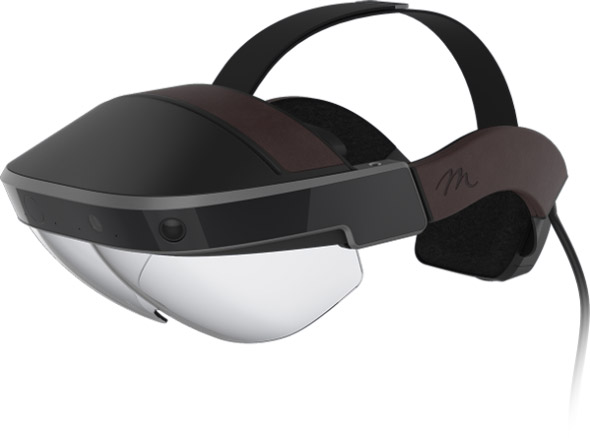
\includegraphics[width=0.66\textwidth]{../images/meta2.jpg}
		\centering
		\caption{Meta 2 - Augmented Reality Glasses}
		\label{fig:SWOT}
\end{figure}

The second class of supported hardware are mobile phones, especially in combination with projects like "Google Cardboard" or Samsung's "Gear VR". These head mounts transform the phones to fully functional augmented reality glasses. 

\begin{figure}[H]
		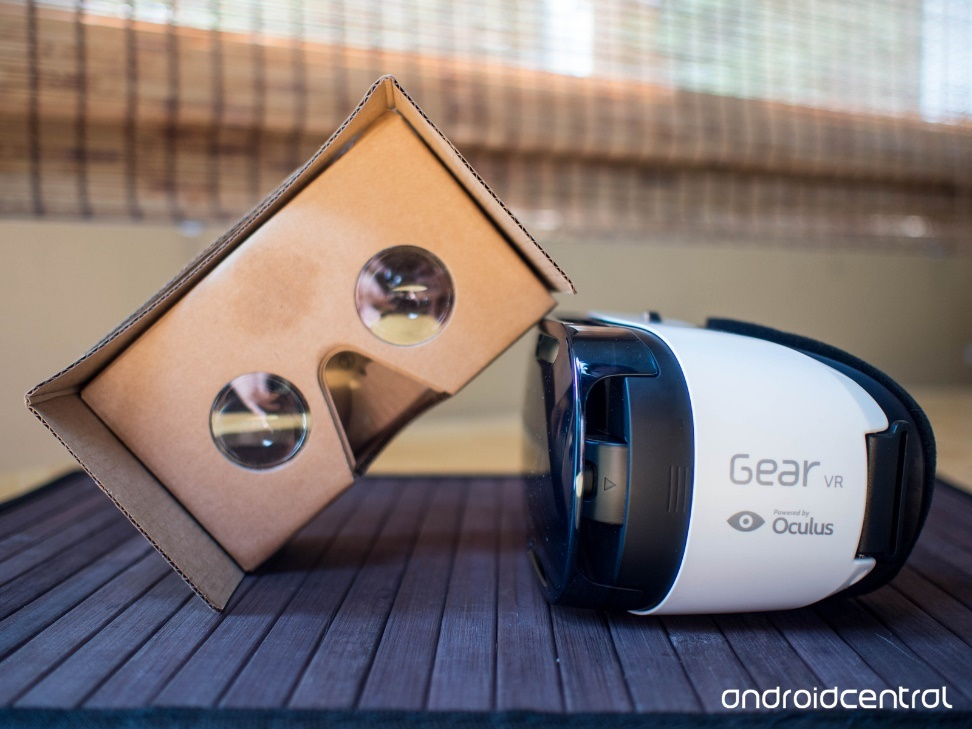
\includegraphics[width=0.66\textwidth]{../images/googleCarboard.jpg}
		\centering
		\caption{Google Cardboard and Gear VR}
		\label{fig:cardBoard}
\end{figure}

The big advantage of mobile phones is, that they are already very common and therefore uFixit can be used  without spending extra money on additional hardware. Modern smart phones also meet the basic requirements for our application, as they already include high resolution cameras, sufficient computational power and a microphone for user input. We would also like to emphasize that devices, which are certified by Google's "Project Tango" are especially suited for uFixit, as those devices provide a depth camera for an even better augmented reality experience.
				

\section{Software}
\subsection{Computer Vison}
To provide the best augmented reality experience possible, it is essential that the virtual objects and annotations of the uFixit manual always remain at the same spatial position they were initially attached to. The software provides two different approaches to find the right locations for the annotations.

The first one uses the camera of the augmented reality glasses to detect the features of the object parts, that are visible to the camera view. The software is now tracking these features from frame to frame throughout the video stream and matches them to the systems internal,  virtual representation of the object. The information about matched feature positions is then used to overlay the annotations provided by the manual onto the users view of the real world.

As uFixit is a platform for repairing broken or deformed parts, it might be impossible for the system to detect the features of the object in question. This is why it is also possible for the creator of a manual to provide positions for optional Fiducial Markers. The fixer prints these markers on paper and attaches them to the specified locations of the broken item. The big advantage of Fiducial Markers is, that compared to object features, the markers have a predefined shape and a limited set of colors. Therefore they are easier to recognize and track by the system.
\begin{figure}[H]
		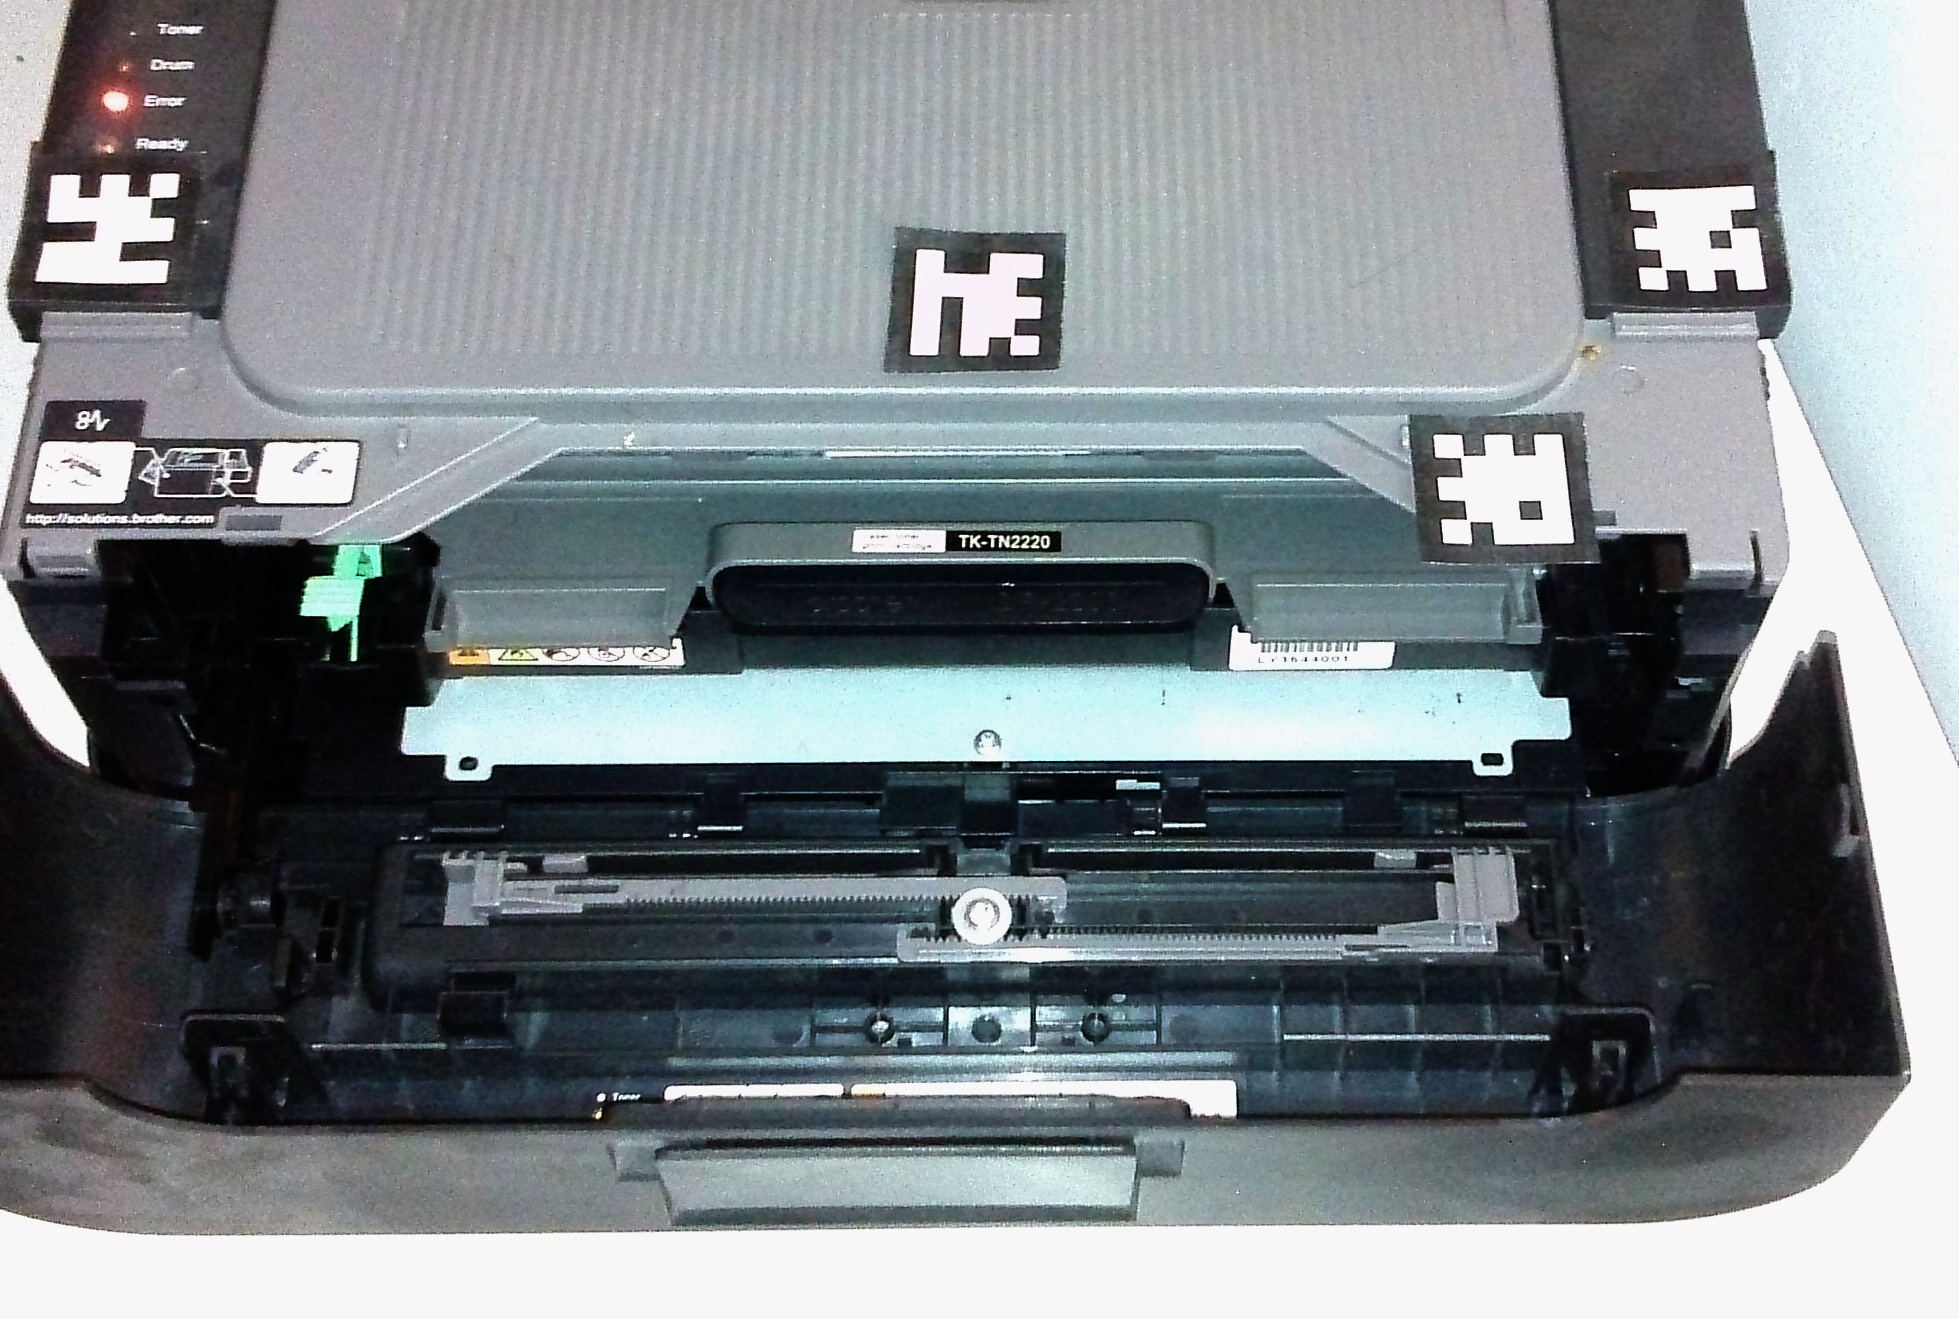
\includegraphics[width=0.66\textwidth]{../images/markerOnObject.jpg}
		\centering
		\caption{Printer with Fiducial Markers at specified positions}
		\label{fig:cardBoard}
\end{figure}

Some objects, like for example watches, are too small for markers to be placed on them. For this scenario, there is an alternative solution, by printing a sheet of paper with markers on its edges. The user then has to position the object, he would like to repair, at a marked position on the sheet. This makes it possible for the system to show an augmentation of the object by tracking the paper sheet with the item being at a known offset to the markers.

\begin{figure}[H]
		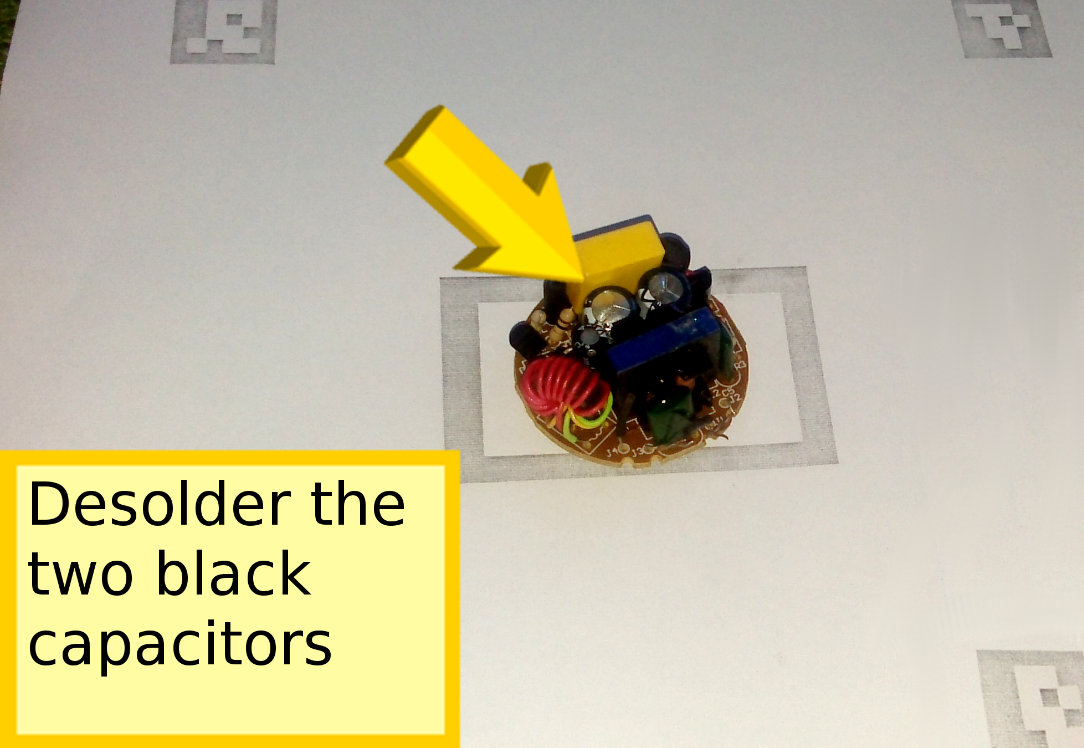
\includegraphics[width=0.66\textwidth]{../images/markerOnPaper.png}
		\centering
		\caption{Small object, centered between Fiducial Markers}
		\label{fig:cardBoard}
\end{figure}

As described in the hardware section \ref{sec:hardware}, uFixit also supports an optional depth camera. This adds the feature of occluded virtual elements to the system. The additional depth information enables the application, to determine the exact distance between the watched item and the AR glasses. Therefore, if an virtual annotation is attached to the other side of the object, uFixit is able to temporarily hide this information from the user until the object is turned around again. This feature helps the user to better understand the spatial relation of the virtual annotations and the real word object.
As this is an optional feature, the application also works without a depth sensor. The only drawback is, that all annotations of the current manual step then are visible at once, even if some of them should be occluded by the object.


\subsection{Manual creation (Manufacturer)}
Instead of shipping paper manuals with their product, uFixit provides an alternative solution for manufacturers. The big advantage of an digital manual is, that errors in the manual or information updated to the product do not require a reprint of the whole manual, but only an update of the uFixit database. Nowadays, industrial products are designed in CAD software like "Solidworks". These softwares packages also provide additional features like animation of the designed items (like rotating screws), creating semi transparent highlighting objects, or adding text objects for explanations. This is why uFixit provides an import interface for industrial instruction creators. This interface is able to import CAD projects and use them as a part of an uFixit manual. Each of the imported snippets then makes up one step of the final instruction set.

\begin{figure}[H]
		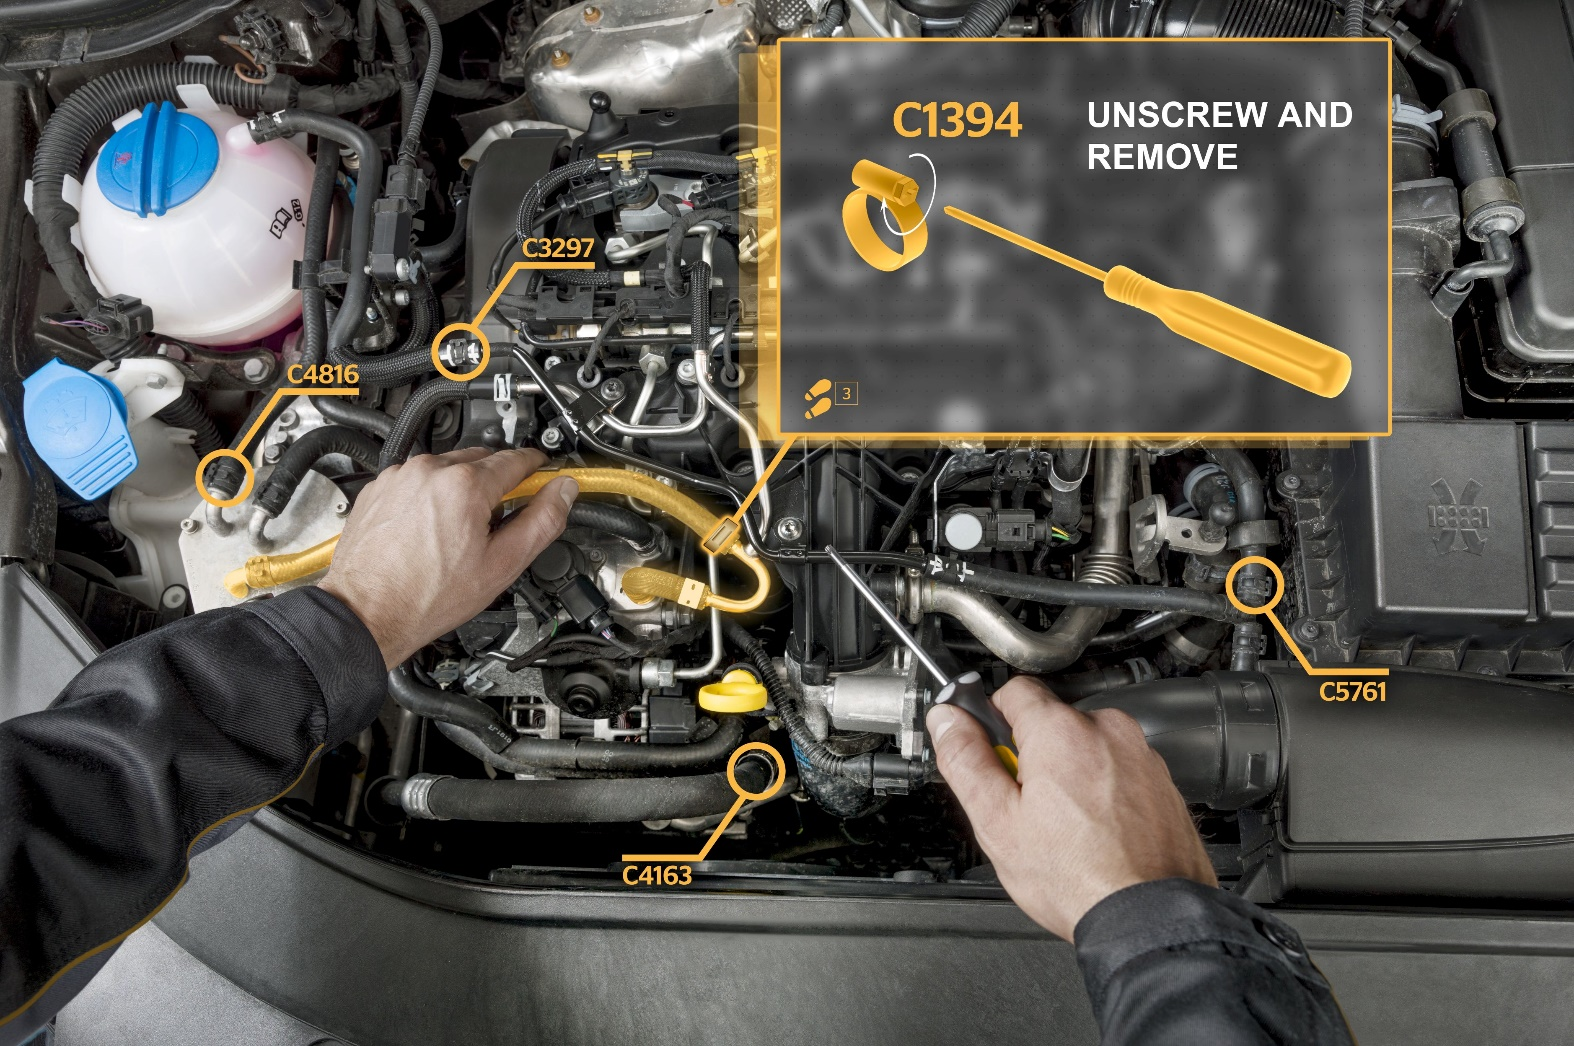
\includegraphics[width=0.66\textwidth]{../images/manufacturer.jpg}
		\centering
		\caption{Manufacturer created uFixit manual}
		\label{fig:cardBoard}
\end{figure}


\subsection{Manual creation (End User)}
Each uFixit user is also able to create own instruction sets and provide them to the community. For the creation, the same hardware is used as for following a manual. The only constraint is, that a depth camera is a requirement for the manual creation. It is important for the precise spatial registration of the manual annotations with the key features of the real world object. For each step of the instruction manual, there are the following annotations possibilities:

\begin{itemize}
\item Arrows
\item Text
\item Highlighting
\item Sketches
\end{itemize}

To annotate items, uFixit uses representations of the annotations in paper form. When paper templates are recognized by the camera, the software adds the corresponding virtual annotation object to the scene. The annotation matches the template's location and also follows the movements of the paper template. 

\begin{figure}[H]
		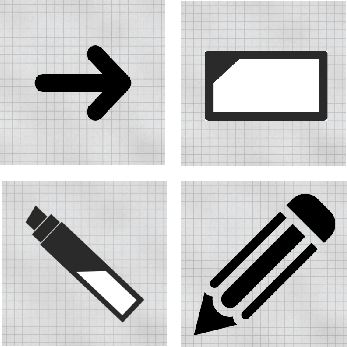
\includegraphics[width=0.66\textwidth]{../images/paperMarker.png}
		\centering
		\caption{Annotation templates}
		\label{fig:cardBoard}
\end{figure}

If for example, an arrow should be added to the current manual step, the following steps are taken:
\begin{enumerate}
\item Holds the printed arrow symbol into the camera view
\item Move the paper until the virtual arrow matches the target position
\item Finalize the position by speech command ("Attach Here")
\end{enumerate}

\begin{figure}[H]
		
\includegraphics[width=0.66\textwidth]{../images/paperArrowAugmented.png}
		\centering
		\caption{Paper template with virtual annotation arrow}
		\label{fig:cardBoard}
\end{figure}

The text annotation is positioned in exactly the same way. After positioning, the text is filled in also using speech recognition. Highlighting and painting with the pen is controlled slightly differently. First, the manual creator moves the tip of the printed highlighter (or pen) at the start position of the annotation. Drawing begins after the "Start drawing" speech command. All locations in the vicinity of the highlighter/pen tip are then annotated until the stop command is given.


\subsection{Live support}
In contrast to the static manuals, the uFixit live support focuses on quick and simple features. Writing annotation texts or creating animations simply takes too much time for the direct communication of the live scenario. This is why the live support limits the possibilities for augmentation to these three features:
\begin{itemize}
\item Arrows
\item Highlighting
\item Audio communication
\end{itemize}

In contrast to all other functions of uFixit, the expert providing live support uses a tablet or PC for the interaction. During the live support, the expert's display shows the camera stream of the AR device. The expert draws and positions the annotations by using a touch screen or mouse.
Due to the visual object tracking by camera, the software is able to anchor the provided visual annotations to their corresponding items. This means, that if the live support highlights specific locations of the camera view, these annotations remain with the object even if the camera view changes.

To avoid scrawly drawings, due to the constantly changing camera view, the camera stream can be frozen. During a frozen stream, annotations are drawn onto one single image of the view, but are still updated in real time into the fixer's augmented view.
% !TeX spellcheck = en_US

\chapter{Possible Business Perspectives}


text


\bibliography{report}

\end{document}
